%*****************************************
% Lab 02: Adder
%*****************************************
\chapter{Adder}\label{add}

\section{Purpose}

This lab builds a simple adder, but the intent is to continue to familiarize students with \LE and how basic arithmetic functions can be completed using simple gate-level logic. Additionally, this lab develops an automated testing system that will be used to test future lab submissions.


\section{Procedure}

Lorem epsum

\subsection{Testing the Circuit}

One way to test this circuit is to use the \textit{poke} tool and click various input combinations for both subcircuits. If the subcircuits are correct then the output will only go high when the correct combination is set on the inputs. However, as digital logic circuits become more complex it is important to automate the testing process so no input combinations are overlooked. \LE includes a \textsc{Simulate -> Test Vector} feature that is used for automating circuit testing.

The first step in using automatic testing is to create a \textit{Test Vector} file. This is a simple \textit{.txt} file that can be created in any text processor, like \textit{Notepad}. \marginpar{Do not use a word processor to create the Test Vector since that would add unneeded codes for things like fonts and margins.} The format for a test vector is fairly simple.

\begin{itemize}
	\item Every line is a single test of the circuit, except the first line.
	\item The first line defines the various inputs and outputs being tested.
	\item Any line that starts with a hash mark (\#) is a comment and is ignored.
\end{itemize}

Following is the test vector file used to test the \lstinline[columns=fixed]|Equation_1| subcircuit.

\begin{Verbatim}[frame=lines,
numbers=left,
xleftmargin=10mm,
xrightmargin=10mm]
# Test vector for Lab 2
# Equation 1
A1 B1 C1 True1
0   0  0     0
0   0  1     0
0   1  0     1
0   1  1     0
1   0  0     1
1   0  1     0
1   1  0     0
1   1  1     1
\end{Verbatim}

Following is an explanation for the \textit{Test vector for Lab 2} file.

\begin{description}
	\item[Line 1] This is just the title of the file. Because this line starts with a hash (\#) it is a comment and will be ignored by \LE.
	\item[Line 2] This is another descriptor line and is ignored by \LE.
	\item[Line 3] This line lists all of the inputs and outputs in the circuit under test. In this case, there are three inputs, \textit{A1}, \textit{B1}, and \textit{C1}, along with one output, \textit{True1}. \LE is able to determine whether the pin is an input or output from its properties. NOTE: each of the inputs and outputs in this circuit are single bits. If an input or output has more than one bit then that must be specified on this line. For example, if \textit{True1} was actually a four-bit output then that pin would be listed as \textit{True1[4]}.
	\item[Line 4] This line contains the first test for the circuit. This line specifies that \LE make \textit{A1}, \textit{B1}, and \textit{C1} equal to zero and then check to be certain that \textit{True1} is also zero.
	\item[Other Lines] All other lines set the three input bits and specify the expected response in the output bit.
\end{description}

The test vector for Equation 2 would look like this:

\begin{Verbatim}[frame=lines,
numbers=left,
xleftmargin=10mm,
xrightmargin=10mm]
# Test vector for Lab 2
# Equation 2
A2 B2 C2 D2 True2
0   0  0  0     0
0   0  0  1     0
0   0  1  0     1
0   0  1  1     0
0   1  0  0     0
0   1  0  1     0
0   1  1  0     0
0   1  1  1     1
1   0  0  0     0
1   0  0  1     0
1   0  1  0     1
1   0  1  1     0
1   1  0  0     0
1   1  0  1     0
1   1  1  0     1
1   1  1  1     0
\end{Verbatim}

In practice, a circuit designer would usually not create two different test vectors but would, instead, create just one file to test all parts of the circuit. Combining the \textit{Equation 1} test and the \textit{Equation 2} test is not quite as easy as appending one after the other since all input and output pins for both circuits must be specified at the top of the file. Following is the test vector for a circuit that combines \textit{Equation 1} and \textit{Equation 2}. Notice that all input and output pins are defined on line three then each line beginning with line four tests both of the equation circuits. Because only eight tests are needed to fully exercise \textit{Equation 1} but 16 are needed for Equation 2, the \textit{Equation 1} tests are repeated starting on Line 12.

\begin{Verbatim}[frame=lines,
numbers=left,
xleftmargin=10mm,
xrightmargin=10mm]
# Test vector for Lab 2
# Equation 1   - Equation 2
A1 B1 C1 True1   A2 B2 C2 D2 True2
0   0  0     0    0  0  0  0     0
0   0  1     0    0  0  0  1     0
0   1  0     1    0  0  1  0     1
0   1  1     0    0  0  1  1     0
1   0  0     1    0  1  0  0     0
1   0  1     0    0  1  0  1     0
1   1  0     0    0  1  1  0     0
1   1  1     1    0  1  1  1     1
0   0  0     0    1  0  0  0     0
0   0  1     0    1  0  0  1     0
0   1  0     1    1  0  1  0     1
0   1  1     0    1  0  1  1     0
1   0  0     1    1  1  0  0     0
1   0  1     0    1  1  0  1     0
1   1  0     0    1  1  1  0     1
1   1  1     1    1  1  1  1     0
\end{Verbatim}

To start a test, click \textsc{Simulate -> Test Vector}. The window illustrated in Figure \ref{fig:add-06} opens. 

\begin{figure}[H]
	\centering
	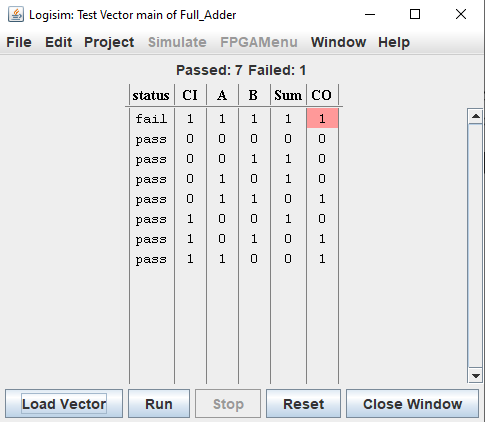
\includegraphics[width=\maxwidth{.95\linewidth}]{gfx/add-06}
	\caption{Test Vector Window}
	\label{fig:add-06}
\end{figure}

Click the \textit{Load Vector} button at the bottom of the window and load the test vector file. The test will automatically start and Logisim-evolution will report the results, like in Figure \ref{fig:add-07}.

\begin{figure}[H]
	\centering
	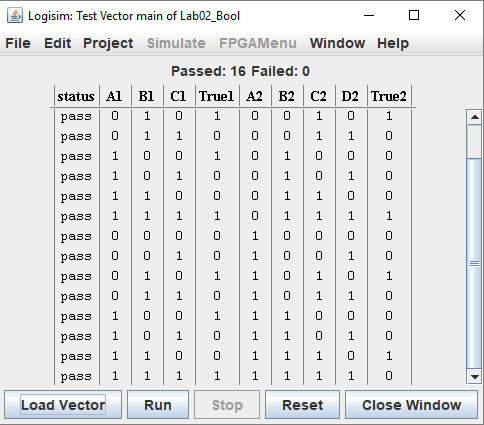
\includegraphics[width=\maxwidth{.95\linewidth}]{gfx/add-07}
	\caption{Test Completed}
	\label{fig:add-07}
\end{figure}

The test indicates all 16 lines passed and zero failed so it could be reasonably concluded that the circuits are functioning properly. Figure \ref{fig:add-08} illustrates a failed test. The circuit designer would then need to troubleshoot to determine what went wrong with the circuit.

\begin{figure}[H]
	\centering
	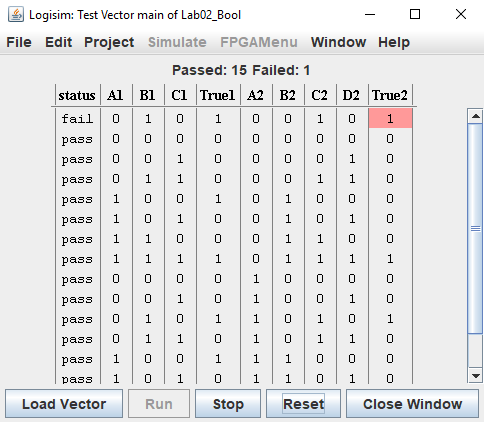
\includegraphics[width=\maxwidth{.95\linewidth}]{gfx/add-08}
	\caption{Test Failure}
	\label{fig:add-08}
\end{figure}


\section{Deliverable}

To receive a grade for this lab, complete the circuit. Be sure the standard identifying information is at the top left of the \lstinline{main} circuit, similar to: 

\bigskip
% The minipage environment keeps the three lines together - no page break.
\begin{minipage}{\linewidth}
	\begin{verbatim}
	George Self
	Lab 02: Adder
	September 17, 2019
	\end{verbatim}
\end{minipage}
\bigskip

Save the file with this name: \emph{\texttt{Lab02\_Adder}} and submit that file for grading.

